\documentclass[../../lecture_notes.tex]{subfiles}

\begin{document}

\noindent Artificial Intelligence is actually one of the oldest fields of computer science.\\
It seeks to understand and build intelligent agents that can:
\begin{enumerate}
	\item Perceive
	\item Understand
	\item Predict
	\item Manipulate
	\item Learn
\end{enumerate}

\noindent These broad goals are shared with philosophy, psychology, neuroscience, etc.\\
\indent BUT we build rational systems, where they seek to understand human ones.\\

\noindent Each specific goal, however, is shared with more computational disciplines:
	\begin{enumerate} [itemsep=0mm]
		\item Perception? Linguistics
		\item Learning? Statistics
		\item Understanding/Prediction? Mathematical Logic
	\end{enumerate}

\noindent The three eras of AI:
\begin{enumerate} [itemsep=0mm]
	\item Knowledge Representation \& Reasoning
		\begin{enumerate} [itemsep=0mm]
        			\item (model): logic
        			\item CS-focused
		\end{enumerate}
	\item Machine Learning
		\begin{enumerate} [itemsep=0mm]
			\item (model \& functions): probability
			\item Statistics and Math-focused
		\end{enumerate}
	\item Neural Networks
		\begin{enumerate} [itemsep=0mm]
			\item (functions): neural networks
			\item Engineering-focused
		\end{enumerate}
\end{enumerate}

\noindent Our initial goals were proposed by Alan Turing; he thus developed \textbf{\underline{The Turing Test:}}\\
\indent $\equiv$ "can an AI convince a human it is human?" This requires:
	\begin{enumerate} [itemsep=0mm]
		\item natural language processing
		\item knowledge representation
		\item automated reasoning
		\item machine learning
	\end{enumerate}
\noindent This avoids physical interaction, so robotics and vision are unneeded.\\
Since we tend to avoid monolithic approaches, this test is not applied nearly as often in the modern day.\\

\noindent \hl{Overview of an AI agent:}
\begin{figure}[H]
	\centering
	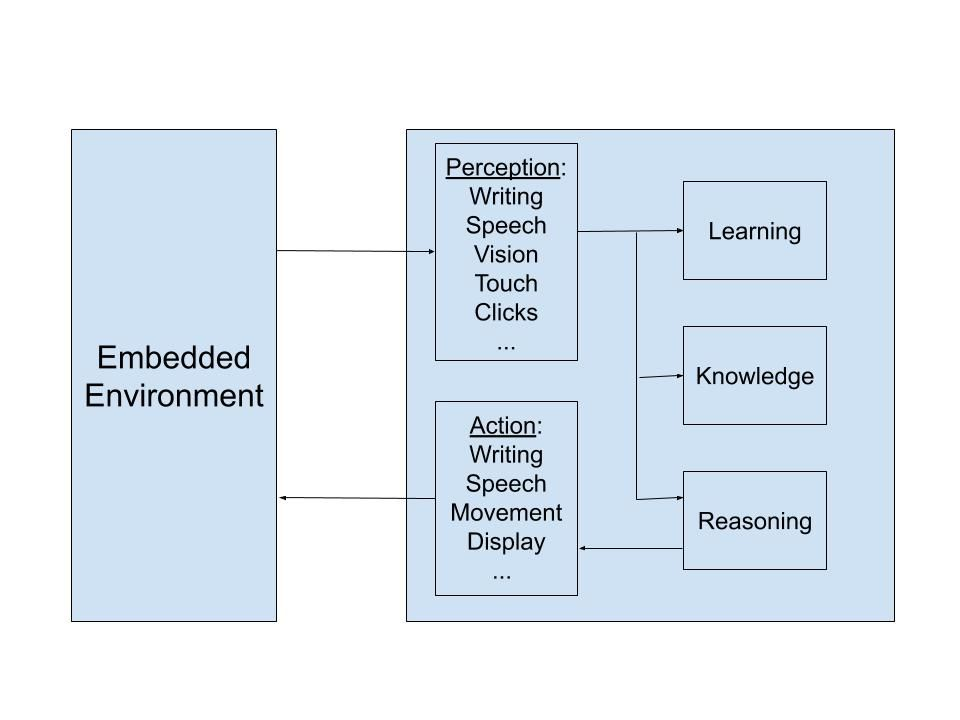
\includegraphics[width=0.6\textwidth]{AI_Overview}
	\caption{a course-grain view of an AI agent}
\end{figure}

\noindent How can we acquire knowledge?
	\begin{enumerate} [itemsep=0mm]
		\item from experts
		\item by conversion from other forms of knowledge
		\item from experience
	\end{enumerate}

How can we categorize knowledge?
\begin{enumerate} [itemsep=0mm]
	\item Uncertain Knowledge (Opinion)
		\begin{enumerate} [itemsep=0mm]
			\item Belief Networks
			\item Fuzzy Logic
		\end{enumerate}
	\item Factual Knowledge (Facts)
		\begin{enumerate} [itemsep=0mm]
			\item Propositional Logic
			\item First Order Logic (if A then B)
		\end{enumerate}
\end{enumerate} \medskip
        

Why do we say A caused B?
\begin{enumerate} [itemsep=0mm]
	\item Needed for explanation
	\item Allows us to predict the future
	\item Suggest ways to control future events
	\item Moral responsibility
	\item Legal liability
\end{enumerate} \medskip

How can we formalize the reasoning process?
\begin{enumerate} [itemsep=0mm]
	\item Deduction: What is implied by a knowledge base?
	\item Belief Revision: What beliefs to prioritize?
	\item Causality: What is the cause of an event?
\end{enumerate} \medskip

\noindent Consider natural language processing:\\
	\indent It involves the following processes:
		\begin{enumerate} [itemsep=0mm]
			\item Understand Natural Language
			\item Generate Natural Language
			\item Text Summarization
			\item Machine Translation
			\item Speech Transcription
		\end{enumerate}
	It has the following complications:
	\begin{enumerate} [itemsep=0mm]
		\item Syntactic Ambiguity: “They are cooking apples”
		\item Semantic Ambiguity: “She ran to the bank”
		\item Pragmatic Ambiguity: “Can you open the door?”
	\end{enumerate}
\noindent We use the following approaches:
\begin{enumerate} [itemsep=0mm]
	\item Classical: 
		\begin{enumerate} [itemsep=0mm]
			\item Provide the system with rich knowledge
			\item Perform the above three types of analysis
			\item Disambiguate using knowledge and reasoning
		\end{enumerate}
	\item Modern:
		\begin{enumerate} [itemsep=0mm]
			\item Rely on corpus (collection of data)
			\item Disambiguate using machine learning
		\end{enumerate}
\end{enumerate} \medskip

\noindent But what is machine learning?\\
\indent $\equiv$ Using experiences and observations to improve future actions\\
\indent Characteristics:
	\begin{enumerate} [itemsep=0mm]
		\item What aspects of performance to be improved?\\
			We must determine and consider:
			\begin{enumerate} [itemsep=0mm]
				\item Irrelevant aspects of the world
				\item How the world evolves
				\item What are desirable/undesirable situations
			\end{enumerate}
		\item What feedback is available?
			\begin{enumerate} [itemsep=0mm]
				\item Supervised: give observations and actions they should lead to
				\item Unsupervised: give observations, machine finds patterns
				\item Reinforcement: give positive/negative feedback on actions
			\end{enumerate}
		\item How to represent output?
			\begin{enumerate} [itemsep=0mm]
				\item Logical Knowledge
				\item Probabilistic Knowledge/Bayesian Networks
				\item Neural Networks
			\end{enumerate}
	\end{enumerate} \medskip
	
\begin{figure}[H]
	\centering
	\includegraphics[width=\textwidth]{Deep_Learning}
	\caption{An example deep learning process}
\end{figure}

\noindent In implementing AI, an important part is \textbf{\underline{planning}}:
	$\equiv$ finding a sequence of actions that will achieve a goal.\\
	\indent We must consider:
	\begin{enumerate} [itemsep=0mm]
		\item Input:
			\begin{enumerate} [itemsep=0mm]
				\item Actions (preconditions, effects)
				\item Initial \& Goal States
				\item Knowledge of world (physics)
			\end{enumerate}
		\item Output:
			\begin{enumerate} [itemsep=0mm]
				\item Conditional/Contingency Plan
				\item Sensorless (Conformant) Approach
				\item Hybrid
			\end{enumerate}
	\end{enumerate} \medskip

\noindent The largest application in the public conscience is \textbf{\underline{robotics}};
	\indent Physical agents that perform tasks by manipulating the world.
	\indent \indent These are equipped with:
		\begin{enumerate} [itemsep=0mm]
			\item Effectors: legs, wheels, joints, grippers
			\item Sensors: cameras, ultrasound, gyroscopes, accelerometers
		\end{enumerate}
    \indent \indent Common categories:
	    \begin{enumerate} [itemsep=0mm]
		\item Manipulators (robot arms): assembly lines, ISS
		\item Mobile robots: unmanned probes/vehicles
		\item Mobile robots with manipulators: humanoid
	\end{enumerate}

\end{document}